\documentclass[a4paper,10pt]{report}
\usepackage[utf8]{inputenc}
\usepackage[pdftex]{graphicx}
\usepackage{wrapfig}

%opening
\title{CM30225 Parallel Computing\\Assessed Coursework Assignment 2\\Report}
\author{Dominic Hauton}

\begin{document}

\maketitle

\begin{abstract}
A report on the advantages and effects of parallelising matrix relaxation using MPI.
\end{abstract}

\section{Code}

The source code is included is structured in three folders:
\begin{itemize}
 \item \emph{matrix} - Responsible for all matrix creation, access and destruction.
 \item \emph{benchmarking} - Contains functions that are used to time and benchmark smooth operations.
 \item \emph{smoothing} - Contains the main loop for for smoothing the matrix.
\end{itemize}
All code is structured using opaque pointers to encapsulate structures and lower coupling, resulting in increased readability and maintainability. Tightly coupled code is often more faster, however, gcc should be able to optimise a lot of function calls.\par
Compilation is done using cmake. The target system must support AVX instructions as Intel Intrinsic Instructions are used for SWAR acceleration.

\section{MPI - Parallelism}

MPI allows for distributed memory parallelism by sending messages between processes. These processes can be run on one or more MPMD (Multiple Program Multiple Data) machine. The scheduler allows these processes to communicate between each other. As each process has it's own local data, there are no issues with concurrent memory access and cache invalidation present in shared memory systems.\par
The presented solution has 3 main stages:
\begin{itemize}
 \item Scatter
 \item Share
 \item Gather
\end{itemize}\par
\subsection{Scatter}
When a matrix is created using \emph{mat\_factory.c} on the master node. It can then be scattered evenly to every process. \emph{MPI\_Scatterv()} is used to allow MPI to decide how best to distribute the information. The original matrix is split into blocks that need to be computed, and an extra row is added above and below. This is then scattered.
\subsection{Share}
After every iteration the data needs to be shared between the processes. Using non-blocking communication allows MPI to schedule incoming and outgoing information itself and means that, depending on the MPI implementation used, these transfers can be performed in parallel, saving time.\par
The compute edge rows (top and bottom rows of the computed block) need to be sent to the process computing the section above and below and placed in their outer edge rows (top and bottom rows of the full matrix). The first and last compute section do not send or update their top and bottom rows respectively.\par
The compute sections need to agree on whether another iteration is required, by ANDing their another computation required flags. If any one section needs to re-smooth, they all need to re-smooth. This is implemented using a \emph{MPI\_Iallreduce()}. This allows MPI to optimise communication between nodes itself and can be done in parallel with the other communication if possible. It also has the benefit of being able to synchronise all of the processes at the end of a loop.
\subsection{Gather}
When all the processes stop needing more iterations all the matrix sections are gathered together and the local matricies are destroyed. Only the computed rows are reassembled at the master node to reduce data throughput required. The MPI command \emph{MPI\_Gatherv()} is used to allow MPI to optimise this operation.
\subsection{Overhead Mitigation}
Three methods of minimise overhead were used:
\subsubsection{Data Reduction}
The data transfered every iteration was minimised to the two required rows and only to the relevant hosts. This resulted in a maximum of 5 transfers per iteration. During the initial scatter all of the data required is sent out in one transaction and in the gather the minimum data required is gathered back in one transaction.
\subsubsection{Native MPI}
The use of native MPI commands such as \emph{MPI\_Scatterv()} utilises the expertise of MPI developers to maximise the performance of the scatter and simplifies the application code. It allows MPI to perform optimisations, such as sending larger data chunks to nodes that are closer, or in the case of \emph{MPI\_Iallreduce()}, allows the reduction and broadcast to happen in a divide and conquer approach.
\subsubsection{Nonblocking MPI}
Using non-blocking MPI commands for the sharing step allows MPI to schedule to communication itself and decide when best to perform tasks such as copying data from the buffer to the pointer for example. This allows communication to be asynchronous and parallel where possible.

\section{Correctness Testing}
\subsection{Sequential vs. Parallel Comparison}
I could assert that my sequential algorithm worked on small sized matrices by printing out the matrix using the mat print function in mat.c. It was easy to observe that all the values in the matrix, which were previously 0.0f, had become very close to the values around the edge of the matrix. Making the assumption that the smoothing function would continue working on larger matrices, I could now compare the results of my parallel calculations to the results of my sequential calculations. To prevent having to recalculate the sequential matrix every time, I created a mat crc64 check that used type punning to interpret the doubles in the matrix as long values and add them. This is much faster than adding doubles. Using a combination of the crc64, parity and the number of times the matrix had been smoothed in the run, I was able to assert the different methods had produced the same values. An sample of the program output is available in the appendix. The CRC and parity should always match that of the sequential version. A print out of a fully smoothed matrix that began as a matrix with zeros on the inside is also available in the appendix along with the calculated CRC.
\subsection{Matrix Symmetry}
I used two ways of testing correctness of the matrix relaxation algorithm. The first was the observation that a matrix that starts with the same number on all the edges, and needs to be smoothed repeatedly will retain the symmetry of the original matrix. Using this known results we now have a method of testing the correctness of the relaxation. In order to check the symmetry I created a function in mat.c called mat parity, which uses type punning to interpret the doubles from the result as long long values, and repeatedly XORs values against each other. If the matrix is indeed symmetric, every single value will be cancelled out by the equal and opposite value on the other side of the matrix.
\subsection{debug\_print()}
I created a macro called debug print, which I used at all times unless I was testing the speed of the code. This along with GDB proved invaluable for stepping through my code and and ensuring the the mutex, spinlocks, semaphores, condition variables and barrier used to synchronise the processes were set to the correct values and that the threads were smoothing the matrix correctly.
\subsection{Timing}
In order to time the program execution, I opted to settle for using wall clock time. Unlike testing this from bash, this allowed me to test smoothing speed in the program without the start-up time for configuring and allocating the matrix. CPU cycles could have been measured, however this value would have been difficult to interpret in a parallel process. The wall clock value may have some error due to leap seconds and load on the system from other processes, however, it proved consistent during testing and gave expected results.

\section{Scalability Investigation}
To conduct my scalability investigation I checked the effect of increasing the problem size and the number of nodes.
\subsection{Methodology}
In order to determine the scalability of the proposed algorithm the time required to smooth the matrix was measured over 5 runs. This time ignores matrix generation time but includes the important initial scatter cost. The matrix generation cost is fixed and irrelevant to the smoothing process and therefore the investigation. This allows the generation to be swapped for a load from file, or even a buffer within the program with no impact on results.

Matrix generation was done from a fixed seed value. To make tests fair the number of smoothing loops required was calculated, and the number of smoothing operations could be calculated by multiplying the inner area of the matrix by smoothing loops.

Each smoothing run printed a line of output which was placed into a spreadsheet and was automatically averaged and using a pivot table various relationships could be plotted. The speedup, efficiency, isoefficiency, overhead, Karp-Flatt metric and processing speed of the solution was calculated within the spreadsheet based on the sequential for each size.

Speed calculation: $$Speed = \frac{Loops * (Matrix\ Size - 2)^2}{Time}$$

Speedup calculation: $$Speedup = \frac{Sequential\ Time}{Parallel\ Time}$$

Efficiency calculation: $$Efficiency = \frac{Speedup}{Processes}$$

Karp-Flatt metric calculation: $$E = \frac{\frac{1}{Speedup} - \frac{1}{Processes}}{1 - \frac{1}{Processes}}$$

Overhead calculation: $$Overhead = Sequential\ Time - (Parallel\ Time + Processes)$$

Isoefficiency calculation: $$Isoefficiency = \frac{1}{1 + \frac{Overhead}{Processes}}$$

These values were then plotted on graphs to explore the relationship of the metrics as conditions changed.
\subsection{Scalability with more Nodes}
The first investigation explores the impact of increasing the number of nodes used to solve the problem.

The speedup of the algorithm should increase with more nodes. There may be a slight decrease in efficiency as more nodes are added, but as all communication is asynchronous there should be a one off cost when the number of nodes goes above one.

To test this the starting matrix was kept constant and the number of processes and nodes was varied. This resulted in four lines showing the speed increase with varying amounts of nodes.

\begin{wrapfigure}{R}{0.6\textwidth}
 \centering
 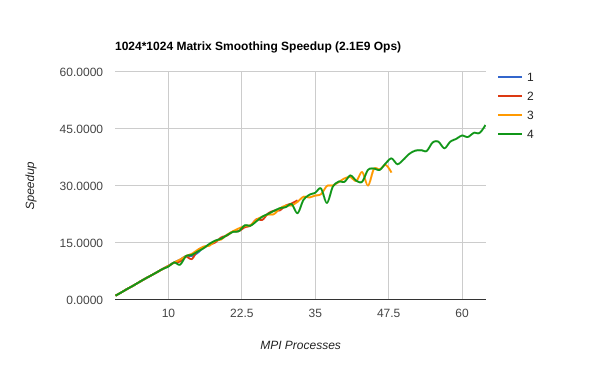
\includegraphics[width=0.6\textwidth]{./images/nodes-speedup.png}
 \caption{Speedup across 1-4 nodes}
 \label{fig:nodespeedup}
\end{wrapfigure}

In figure \ref{fig:nodespeedup} we can see the speedup increasing constantly with a very slight fluctuation when the mpirun was required to run the process on more cores than there were available on one node. However, the impact of this change is very small, much smaller than the noise seen as more processes are used across 3-4 nodes. This is indicative of a very small and constant communication overhead, which does not change if more than one node is used. This may be a sign that MPI is using message passing to communicate between processing instead of memcpy even when on the same node.

\begin{wrapfigure}{L}{0.6\textwidth}
 \centering
 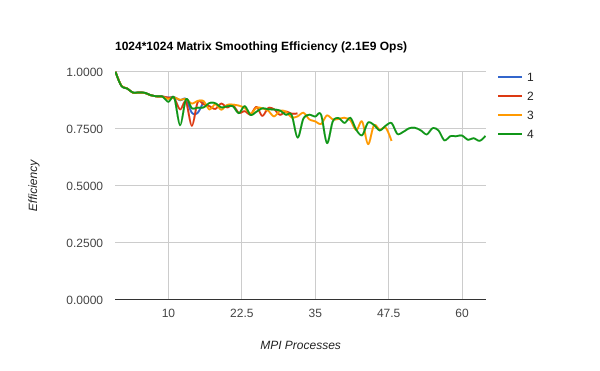
\includegraphics[width=0.6\textwidth]{./images/nodes-efficiency.png}
 \caption{Efficiency across 1-4 nodes}
 \label{fig:nodeefficiency}
\end{wrapfigure}

In the efficiency graph in figure \ref{fig:nodeefficiency} we can see that fairly constant efficiency drop-off as more processes were used, but again no sudden drop off as more nodes were added. This is consistent with the idea that while the communication time is kept constant, there is less and less to do in parallel, so efficiency in the constant time communication lowers the efficiency.

A key observation is that efficiency remains consistent for the same number of MPI processes, regardless of nodes used. This is indicative of mpirun correctly scheduling processes on as few nodes as possible.

As a result of this investigation we can see that the number of nodes does not substantially effect the speed of the algorithm when the number of MPI processes are kept the same. Following this we shall now use 4 nodes during experiments.

\subsection{Scalability with larger matrix}
I second investigation tackles scaling the problem and will also explore different metrics of measuring scalability.

\begin{wrapfigure}{R}{0.5\textwidth}
 \centering
 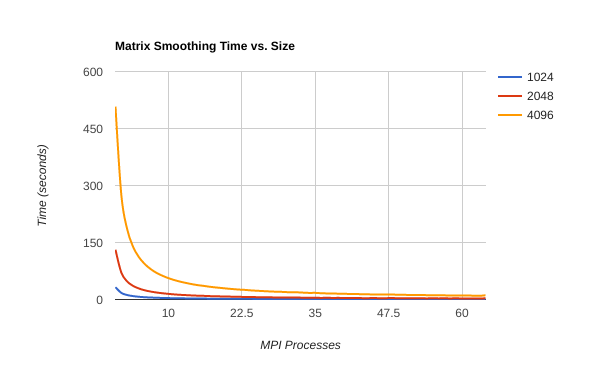
\includegraphics[width=0.5\textwidth]{./images/sizes-time.png}
 \caption{Time across 3 matrix sizes}
 \label{fig:sizestime}
\end{wrapfigure}

According to Gustafson, the speedup of the algorithm should increase as the size of the problem increases. To investigate three sizes of matrix were chosen, each in serial taking four times the length of time that the one before took. A seed for the matrix was chosen that resulted in roughly the same time, and when comparing between matrices of different sizes, we can use the speed metric.

In figure \ref{fig:sizestime} we can see the computation time decreasing, following the curve of a rational function. This is expected in a parallel algorithm. To be able to observe how fast the nodes are actually processing data, we need to look at the raw processing speed. We use the speed equation to find how many smoothing operations had to be done for the smooth to complete.

\begin{wrapfigure}{L}{0.5\textwidth}
 \centering
 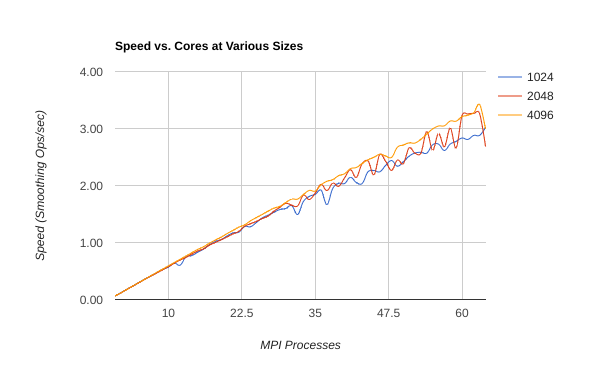
\includegraphics[width=0.5\textwidth]{./images/sizes-speed.png}
 \caption{Efficiency across 3 matrix sizes}
 \label{fig:sizespeed}
\end{wrapfigure}

Figure \ref{fig:sizespeed} gives us our first glimpse of two important trends in the data. Larger data sets tend run at a faster speed, more calculations are done per second while the algorithm is running, and this discrepancy grows as more MPI processes are used. This is most likely due to the fact that individual cores need to stop less often for reductions and can run at a faster speed because of it.

\begin{wrapfigure}{R}{0.5\textwidth}
 \centering
 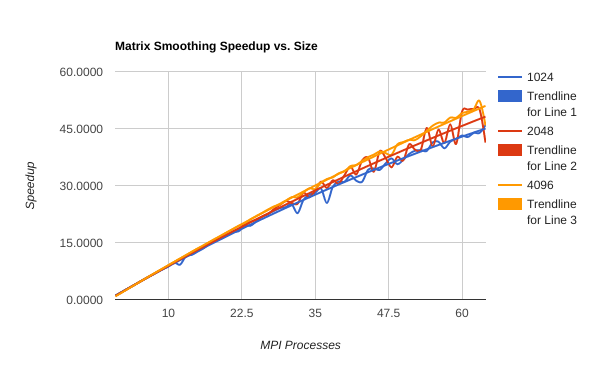
\includegraphics[width=0.5\textwidth]{./images/sizes-speedup.png}
 \caption{Speedup across 3 matrix sizes}
 \label{fig:sizespeedup}
\end{wrapfigure}

To explore this relationship further the speedup was also plotted in figure \ref{fig:sizespeedup}. This follows the same trend as the raw speed, but now showing it in terms of the original sequential speed. Using the 





In order to see how worthwhile it is to run the function on multiple cores, we need to look at the efficiency of the algorithm. The efficiency usually ignores the problem size and focuses on scaling for that specific size. In figure \ref{fig:sizesefficiency} we see efficiency following the expected trend. Trend lines are added to show the pattern more clearly as the data is noisy.

\begin{wrapfigure}{R}{0.6\textwidth}
 \centering
 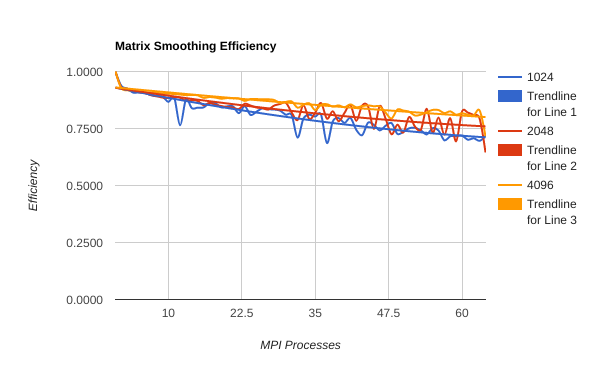
\includegraphics[width=0.6\textwidth]{./images/sizes-efficiency.png}
 \caption{Efficiency across 3 matrix sizes}
 \label{fig:sizesefficiency}
\end{wrapfigure}






\section{Other Parallelism}
\subsection{MPI \& Thread Pooling}
\subsection{SWAR}

\end{document}
